\section{関連研究}

基本的にドローンが自律飛行を行う際に必要とされる処理がいくつかある.そのうちの2つが自己位置推定と姿勢推定である.
自己位置推定とは,ドローンが飛行している空間の中で自分がどの位置にいるのかを認識する事である.姿勢推定とは自分が水平方向に対してどの程度傾いているのか,鉛直方向に対してどの程度回転しているかといった事を認識することある.

これらを行なっている関連研究としてNanomap\cite{Nanomap}という飛行モデルがある.においては2D-LIDARを用いた飛行経路探索手法が取られており,取得した点群データを過去数フレーム分を記憶しておき,過去の数フレーム分のデータと現在のフレームとの点群の変量によっておおよその障害物の位置を認識している.こちらの手法では,物体を正確に捉えることは放棄し,不確実な部分を物体の存在している可能性のある範囲として捉えている.視野にある物体のある可能性も含めて1番物体が少ない方向を飛行経路として選定し,飛行している.

他に,ドローンに限らずロボット工学全般で利用されてきたOctomap\cite{Octomap}がある.
こちらもNanomapと同様にLIDARを用いて周辺の環境情報を扱うものであるが,こちらはLIDARを用いて実際に周囲を点群からモデリングして周辺状況を把握する.

Octomapではモデリングする際に近い点群同士を同じ物体としてまとめ1つのブロックにするということを繰り返し,樹構造的にブロックを生成する為,生成後のデータは繰り返す回数等のパラメータによっては小さく圧縮することもできる.
\begin{figure}[htbp]
  \begin{center}
    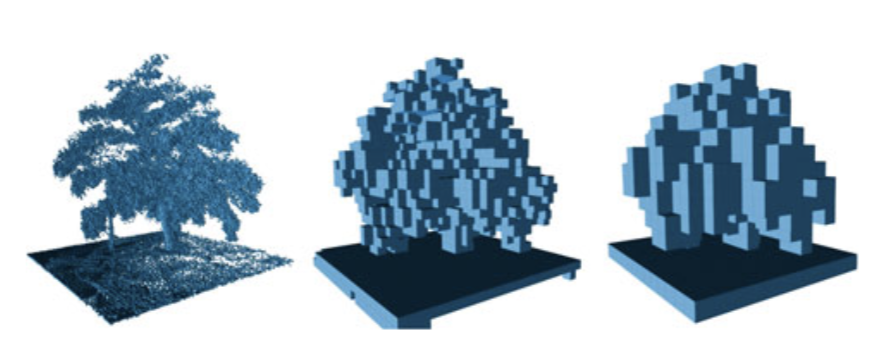
\includegraphics[clip,width=7.0cm]{img/octomap.png}
    \caption{圧縮率の違いによる生成物の違い}
    \label{fig:hamu}
  \end{center}
\end{figure}
しかし,実際に点群からモデルを生成するとなるとその計算量は非常に多く,高性能な小型コンピュータが現れている現在においても処理負荷が大きく,特にドローンにおいては積載量に制限がかかりやすい為扱いにくいものとなっている.


また,これらのようにLIDARを使用せず,CMOSセンサーのみで自律飛行を行なっている例もある.

実用性を備えた手のひらサイズ・完全オンボード処理 UAV のための 3 次元自己位置推定手法の提案と全自動飛行の実現\cite{SfMDrone}では自己位置推定で使用するセンサーはCMOSセンサーを利用した自律飛行を実現している.
CMOSセンサーからの映像をFPGAにストリームしてFAST\cite{FAST}による特徴点抽出処理を行い,その結果をBrief\cite{Brief}を用いて表現し,MCUに流し込み処理している.この研究での目的は外部処理系に依存せず,ドローン上で全て完結する自律飛行可能な小型ドローンの開発で,限定条件下(新聞紙を敷き詰めた床面)の上で飛行させ,特徴点を十分に検出できるようにした上で,飛行させ想定通りの飛行を実現している.

他に今回の研究のベース物としてDeepDrone\cite{DeepDrone}が挙げられる.こちらではドローンレースを自律飛行で行う為に自律飛行モデルを提案している.ドローンレースとは基本的にゲートを順に潜りながら飛行することが条件となっているドローン競技である.このゲートをRGBカメラで撮影した映像を推定モデルに対し,200*300の画像を所与として$\lbrace \vec{x}, v \rbrace$,を推定結果として得る.$\lbrace \vec{x}$は$\vec{x} \in [-1,1]^2$と定義され正規化された入力画像の中にある目標とするゲートへの方向を表していおり, $v \in [0,1]$ は飛行速度を正規化して表している.

DeepDroneでは訓練にシミュレータでのデータと現実世界でのデータを使っている.両者とも理想とする軌道とのズレを計算しそのズレを損失関数に入力し学習を進めていく.
\begin{figure}[htbp]
  \begin{center}
    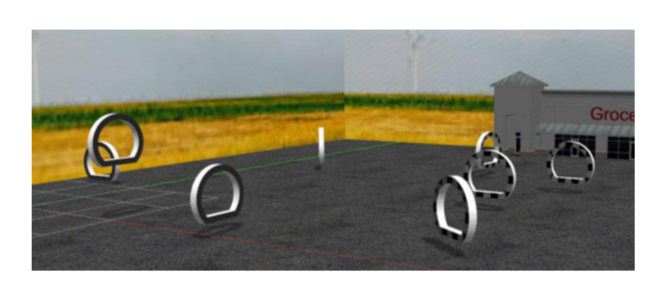
\includegraphics[clip,width=7.0cm]{img/deep-simu.png}
    \caption{シミュレータ上のゲート}
    \label{fig:gate}
  \end{center}
\end{figure}
シミュレータ上では直接理想とする軌道とのズレを取得し,実空間では実際に手動で実際のコース上を運び,ゲートを通過させるなどしてデータを収集していた.

他に屋内でドローンの位置測位を行っている例としてScalable and Precise Multi-UAV Indoor Navigation\cite{TDOA-UWB}が挙げられる。これはTDOA-UWBという方式を用いたものである。TDOA(Time Differences of Arrival)とは電波を用いた位置推定手法でありTOA(Time of Arrival)とよく比較される。Time of Arrivalでは電波を発信する送信機と位置推定を行う受信機との構成で行われる。送信機と受信機で時刻同期を行った上で、各送信機からの伝播時間を計測。この電波時間から距離を計算し、複数の送信機を用いると位置推定を行う事が出来る。

一方でTDOAでは時刻同期の必要はなく、送信されてくる電波の時間差を用いて位置推定を行う。
今回挙げているこの例ではTDOAによる位置測位を行うのにUWBを電波として用いている。


